\documentclass[parskip=full]{scrartcl}
\usepackage[utf8]{inputenc} % use utf8 file encoding for TeX sources
\usepackage[T1]{fontenc}    % avoid garbled Unicode text in pdf
\usepackage[german]{babel}  % german hyphenation, quotes, etc
\usepackage{hyperref}       % detailed hyperlink/pdf configuration
\hypersetup{                % ‘texdoc hyperref‘ for options
pdftitle={Aufgabe_1},%
bookmarks=true,%
}
\usepackage{graphicx}       % provides commands for including figures
\usepackage{csquotes}       % provides \enquote{} macro for "quotes"
\usepackage[nonumberlist]{glossaries}     % provides glossary commands
\usepackage{enumitem}

\makenoidxglossaries
%
% % Glossareinträge
%
\newglossaryentry{Benutzern}
{
	name=Benutzer,
	plural=Benutzer,
	description={jemand, der etwas [leihweise] benutzt},
}

\newglossaryentry{Komprimierung}
{
	name=Komprimierung,
	description={Datenkomprimierung ist eine Reduzierung der Anzahl von Bits, die zur Darstellung von Daten benötigt werden.}
}
\newglossaryentry{Kunstfiltern}
{
	name=Kunstfilter,
	plural=Kunstfiltern,
	description={Funktion in einer Grafiksoftware, die ein bestehendes digitales Bild (meistens Rastergrafik) mit einem vorprogrammierten Algorithmus, der häufig in einigen Parametern konfigurierbar ist, gezielt verändern}
}

\newglossaryentry{Metainformationen}
{
	name=Metainformation,
	plural=Metainformationen,
	description={Information, die anderer Information übergeordnet ist}
}

\newglossaryentry{Server}
{
	name=Server,
	plural=Server,
	description={Rechner, der für andere in einem Netzwerk mit ihm verbundene Systeme bestimmte Aufgaben übernimmt und von dem diese ganz oder teilweise abhängig sind}
}

\newglossaryentry{Rechner}
{
	name=Rechner,
	description={Gerät zur Verarbeitung zur Daten, das die Daten einlesen, verarbeiten, speichern und ausgeben kann}
}

\title{iMage: Lastenheft}
\author{Kaloyan Draganov, 2313306}

\begin{document}

\maketitle

\section{Zielbestimmung}
Die Firma Pearcorp entwickelt das System iMage. iMage ist ein Bildverarbeitungssoftware Produkt mit Schwerpunkt auf \gls{Kunstfiltern}. Dem \gls{Benutzern} wird die Möglichkeit zur Verfügung gestellt, im Internet nach frei nutzbare Bilder zu suchen, sie zu bearbeiten und auf dem lokalen \gls{Rechner} oder auf dem Pearcorp \gls{Server} zu speichern.

\section{Produkteinsatz}
Das Produkt dient zur Bilderorganisation und Bilderberarbeitungszwecke.

Zielgruppe: die Kunden der Firma Pearcorp.

Plattform: PC mit Windows 7 oder Nachfolger-Betriebssystem.

\section{Funktionale Anforderungen}
\begin{itemize}[nosep]
\item[FA10] Internetsuche für Bilder nach einer angegebenen Reihe von Schlüsselwörter.
\item[FA20] Anzeigen von zuletzt zugegriffenen Bilder.
\item[FA30] Lokales Speichern von ausgewählten Bilder.
\item[FA40] Entferntes Speichern von ausgewählten Bilder auf einem zum System zugehörigen Zentralserver.
\item[FA50] Komprimierung von Bilddateien.
\end{itemize}

\section{Produktdaten}
\begin{itemize}[nosep]
\item[PD10] Es sind vom Benutzer ausgewählten Bilder zu speichern.
\item[PD20] Es sind zum Bilder gehörige \gls{Metainformationen} zu speichern. Insbesondere zählen dazu Nutzungsrechte.
\item[PD30] Es sind Kontodaten des Benutzers, insbesondere für Organisation der Verzeichnisbaum des Servers, zu speichern.
\end{itemize}

\section{Nichtfunktionale Anforderungen}
\begin{itemize}[nosep]
\item[NF10] Die Suche soll für eine Anzahl von fünfhundert (500) Bildern maximal zehn (10)Minuten benötigen und selbstständig nach einer Suchdauer von einer Stunde abbrechen.
\item[NF20] Maximal sollen 50  Bilder  gleichzeitig  angezeigt  werden.
\item[NF30] Der Zugriff auf den Zentralserver soll von mindestens einhundert (100) Nutzern gleich-zeitig erfolgen können.
\item[NF40] Die Dauer des Hochladens der Bilder darf maximal linear mit der Anzahl der Bilder wachsen.
\item[NF50] Der maximale Grad an \gls{Komprimierung} soll dabei abhängig von der Bildgröße so berechnet werden, dass die Motive in 90\% der Bilder erkennbar bleiben.
\end{itemize}

\section{Systemmodelle}

\subsection{Anwendungsfälle}
\begin{center}
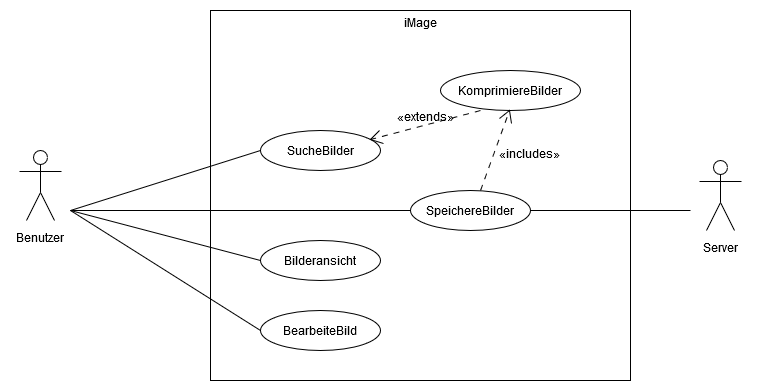
\includegraphics[width=0.8\textwidth]{iMage_Anwendungsfalldiagramm.png}
\end{center}

Akteure: Benutzer, Server.

Anwendungsfälle: SucheBilder, Bilderansicht , BearbeiteBild, SpeichereBilder, KomprimiereBilder.

\subsubsection{Anwendungsfall: "`SucheBilder"'}

Teilnehmende Akteure: Benutzer

Ereignisfluss:

\begin{itemize}[nosep]
\item Der Benutzer aktiviert die Suchfunktion des Systems(entweder mit oder ohne Komprimierung). iMage öffnet ein Auswahlfenster mit verschiedenen Suchoptionen.
\item Der Benutzer gibt die Suchparameter ein und tätigt die BilderSuche. Er gibt ebenso die Domänen in denen die Suche vorgenommen werden soll. iMage sucht nach den Parameter im Internet und liefert die Ergebnisse den Benutzern.
\end{itemize}

\subsubsection{Anwendungsfall: "`Bilderansicht"'}

Teilnehmende Akteure: Benutzer

Ereignisfluss:

\begin{itemize}[nosep]
\item Der Benutzer tätigt das Anzeigen des letzten Bild nach einer Bildersuche oder wählt die Option für Bilderanzeigen der Benutzeroberfläche des Systems. iMage lädt den Bildschirm für das Anzeigen von Bilder und stellt die letzten (falls vorhanden bis maximal 50) Bilder dar.
\item Der Benutzer wählt Bilder für Bearbeitung oder für Speichern aus.
\end{itemize}

\subsubsection{Anwendungsfall: "`BearbeiteBild"'}

Teilnehmende Akteure: Benutzer

Eingangsaktionen: Der Benutzer hat ein Bild für Bearbeitung aus dem allgemeinen Ansicht ausgewählt.

Ereignisfluss:

\begin{itemize}[nosep]
\item Der Benutzer wählt die Bearbeitungsoption der Benutzeroberfläche des Systems. iMage öffnet ein Auswahlfenster mit verschiedenen Bearbeitungsoptionen.
\item Der Benutzer wählt eine Option aus und fordert deren Ausführung. iMage wendt den zugehörigen Kunstfilter auf dem Bild an und liefert das Ergebnis den Benutzern.
\end{itemize}

\subsubsection{Anwendungsfall: "`SpeichereBilder"'}

Teilnehmende Akteure: Benutzer, Server

Eingangsaktionen: Der Benutzer hat ein oder mehrere Bilder für Speichern aus dem allgemeinen Ansicht ausgewählt oder hat ein Bild erfolgreich bearbeitet. Fürs Speichern auf dem Server ist eine Internetverbindung erforderlich.

Ereignisfluss:

\begin{itemize}[nosep]
\item Der Benutzer wählt die Speichernoption der Benutzeroberfläche des Systems. iMage öffnet ein Auswahlfenster mit zwei Speicheroptionen: lokales Speichern oder Speichern auf dem Server.
\item Der Benutzer wählt eine Option aus und muss beim lokalen Speichern einen gültigen Verzeichnichpfad angeben. Beim Speichern auf dem Server übernimmt iMage das Verzeichnismanagement. iMage speichert das/die Bilder.
\item Im Fall eines Speichern auf dem Server sendet iMage den Server eine Speichernanforderung mit den Kontodaten des Benutzers. Der Server bestätigt das Konto des Benutzers und iMage sendet das/die Bild/er fürs Speichern. Der Server durchführt das Speichern und informiert iMage über der Abschließung der Prozedur.
\item Der Benutzer bekommt eine Bestätigung vom System fürs erfolgreiche Speichern.
\end{itemize}

\subsubsection{Anwendungsfall: "`KomprimiereBilder"'}

Teilnehmende Akteure: Benutzer

Eingangsaktionen: Der Benutzer hat eine Suche mit Komprimierung oder Speichern auf dem Server getätigt.

Ereignisfluss:

\begin{itemize}[nosep]
\item Nachdem der Benutzer eine Suche mit Komprimierung oder Speichern auf dem Server getätigt hat nimmt iMage eine Komprimierung vor.
\item Die Komprimierung wird von iMage intern durchgeführt und das System läuft automatisch nach dem nächsten Zustand. Die komprimierte Bilderdateien ersetzen die Originaldateien.
\end{itemize}

%
% % Automatisch generiertes Glossar (Latex zwei mal ausführen um Glossar anzuzeigen)
%
%\glsaddall % das sorgt dafür, dass alles Glossareinträge gedruckt werden, nicht nur die verwendeten. Das sollte nicht nötig sein!
\printnoidxglossaries


\end{document}
